\chapter{Hypothesis Testing (Non-Parametric)}

Previously, we examined tests that require certain assumptions about the underlying distribution from which the data arises. Tests which do not require such assumptions are called \emph{non-parametric}. Note that non-parametric tests are generally less powerful than the equivalent parametric tests, especially if the assumptions required by the parametric tests can be justified.

\section{Sign Test}

\subsection{Single Sample}

Consider a random sample of size $n$ from a population which has a continuous distribution with median $m$. We are interested in whether the median $m$ takes on a particular value $m_0$. That is, we are interested in testing the null hypothesis \[\nullhyp: \, m = m_0\] against any of the possible alternative hypotheses: \[\althyp: \, m > m_0 \quad \althyp: \, m < m_0 \quad \althyp: \, m \neq m_0.\]

Define $K_+$ to be the number of data values greater than $m_0$, and $K_-$ to be the number of data values smaller than $m_0$. Under \nullhyp, we expect about the same number of data values that are greater than $m_0$ and less than $m_0$.

\begin{center}\tikzsetnextfilename{493}
    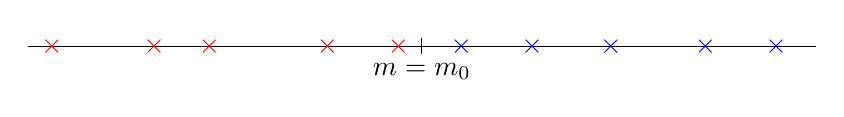
\begin{tikzpicture}
        \draw (-5, 0) -- (5, 0);
        \draw (0, 0.1) -- (0, -0.1) node[anchor=north] {$m = m_0$};
        \draw (-4.7, 0) node[red]{$\times$};
        \draw (-3.4, 0) node[red]{$\times$};
        \draw (-2.7, 0) node[red]{$\times$};
        \draw (-1.2, 0) node[red]{$\times$};
        \draw (-0.3, 0) node[red]{$\times$};
        \draw (0.5, 0) node[blue]{$\times$};
        \draw (1.4, 0) node[blue]{$\times$};
        \draw (2.4, 0) node[blue]{$\times$};
        \draw (3.6, 0) node[blue]{$\times$};
        \draw (4.5, 0) node[blue]{$\times$};
    \end{tikzpicture}
\end{center}

Hence, our test statistic is either \[K_+ \sim \Binom{n}{\frac12} \quad \tor \quad K_- \sim \Binom{n}{\frac12},\] depending on which is more convenient. For now, we take $K_+$ to be our test statistic.

If we test \nullhyp{} against \althyp: $m > m_0$, then we reject \nullhyp{} if the observed number of data values greater than $m_0$ is too large, i.e. $k_+ \geq c_+$ for some critical value $c_+$. Alternatively, we can consider the $p$-value, which is given by $\P{K_+ \geq k_+}$. If this $p$-value is smaller than our significance level $\a$, we reject \nullhyp.

\begin{center}\tikzsetnextfilename{494}
    \begin{tikzpicture}
        \draw (-5, 0) -- (5, 0);
        \draw (0, 0.1) -- (0, -0.1) node[anchor=north] {$m$};
        \draw (-3, 0.1) -- (-3, -0.1) node[anchor=north] {$m_0$};

        \draw (-4.7, 0) node[red]{$\times$};
        \draw (-3.4, 0) node[red]{$\times$};
        \draw (-2.7, 0) node[blue]{$\times$};
        \draw (-1.2, 0) node[blue]{$\times$};
        \draw (-0.3, 0) node[blue]{$\times$};
        \draw (0.5, 0) node[blue]{$\times$};
        \draw (1.4, 0) node[blue]{$\times$};
        \draw (2.4, 0) node[blue]{$\times$};
        \draw (3.6, 0) node[blue]{$\times$};
        \draw (4.5, 0) node[blue]{$\times$};
    \end{tikzpicture}
\end{center}

If we test \nullhyp{} against \althyp: $m < m_0$, then we reject \nullhyp{} if the observed $k_+$ is too small. Alternatively, if the $p$-value $\P{K_+ \leq k_+}$ is smaller than our significance level $\a$, we reject \nullhyp.

\begin{center}\tikzsetnextfilename{495}
    \begin{tikzpicture}
        \draw (-5, 0) -- (5, 0);
        \draw (0, 0.1) -- (0, -0.1) node[anchor=north] {$m$};
        \draw (3, 0.1) -- (3, -0.1) node[anchor=north] {$m_0$};

        \draw (-4.7, 0) node[red]{$\times$};
        \draw (-3.4, 0) node[red]{$\times$};
        \draw (-2.7, 0) node[red]{$\times$};
        \draw (-1.2, 0) node[red]{$\times$};
        \draw (-0.3, 0) node[red]{$\times$};
        \draw (0.5, 0) node[red]{$\times$};
        \draw (1.4, 0) node[red]{$\times$};
        \draw (2.4, 0) node[red]{$\times$};
        \draw (3.6, 0) node[blue]{$\times$};
        \draw (4.5, 0) node[blue]{$\times$};
    \end{tikzpicture}
\end{center}

Lastly, if we test \nullhyp{} against \althyp: $m \neq m_0$, then we reject \nullhyp{} if the observed $k_+$ is too small or too large. In this case, the $p$-value is given by \[2 \min{\P{K_+ \geq k_+}, \P{K_+ \leq k_+}}.\] Note that we choose the shorter tail since we want the more ``extreme'' end.

To summarize, 

\begin{table}[H]
\centering
    \begin{tabular}{|c|ccc|}
        \hline
        \textbf{\nullhyp} & \multicolumn{3}{c|}{$m = m_0$} \\ \hline
        \textbf{\althyp} & \multicolumn{1}{c|}{$m > m_0$} & \multicolumn{1}{c|}{$m < m_0$} & $m \neq m_0$ \\ \hline
        \textbf{$p$-value ($K_+$)} & \multicolumn{1}{c|}{$\P{K_+ \geq k_+}$} & \multicolumn{1}{c|}{$\P{K_+ \leq k_+}$} & $2\min{\P{K_+ \geq k_+}, \P{K_+ \leq k_+}}$ \\ \hline
        \textbf{$p$-value ($K_-$)} & \multicolumn{1}{c|}{$\P{K_- \leq k_-}$} & \multicolumn{1}{c|}{$\P{K_- \geq k_-}$} & $2\min{\P{K_- \geq k_-}, \P{K_- \leq k_-}}$ \\ \hline
    \end{tabular}
\end{table}

In the case where there are zeroes, we discard them and reduce the sample size accordingly.

\begin{sample}
    The lifetimes of a random sample of candles, measured in minutes are \[354, \quad 358, \quad 348, \quad 342, \quad 352, \quad 335, \quad 364, \quad 345, \quad 360, \quad 341.\] The manufacturer claims that the median lifetime is at least 360 minutes. Use a sign test, at the 5\% significance level, to test whether the manufacturer's claim is justified.
\end{sample}
\begin{sampans}
    Let $m$ be the population median. Our hypotheses are \nullhyp: $m = 360$ and \althyp: $m < 360$. We take a 5\% level of significance. Subtracting the observed data values by the postulated median $m = 360$ and writing down the signs, we obtain \[-, \quad -, \quad -, \quad -, \quad -, \quad -, \quad +, \quad -, \quad 0, \quad -.\] Let $K_+$ be the number of data values greater than 360. Discarding the zero, we have, under \nullhyp, $K_+ \sim \Binom{9}{1/2}$. From the sample, $k_+ = 1$. The $p$-value is hence $\P{K_+ \leq 1} = 0.0195$. Since the $p$-value is smaller than our 5\% significance level, we reject \nullhyp{} and conclude there is sufficient evidence at the 5\% level that the manufacturer's claim is not justified.
\end{sampans}

\subsection{Paired Sample}

By considering the difference in population medians, the sign test can be used for paired samples, as demonstrated in the example below.

\begin{sample}
    Students in a school take a mock examination before taking the actual A-level examination. The marks for a particular subject, in both the mock and actual examinations, by a random sample of 13 students are shown below.

    \begin{table}[H]
        \centering
        \begin{tabular}{|r|c|c|c|c|c|c|c|c|c|c|c|c|c|}
            \hline
            \textbf{Candidate Number} & 1 & 2 & 3 & 4 & 5 & 6 & 7 & 8 & 9 & 10 & 11 & 12 & 13 \\ \hline
            \textbf{Mock Exam Mark} & 40 & 65 & 53 & 79 & 87 & 42 & 80 & 63 & 51 & 82 & 27 & 71 & 29 \\ \hline
            \textbf{Actual Exam Mark} & 45 & 68 & 47 & 75 & 88 & 60 & 77 & 69 & 60 & 88 & 30 & 73 & 35 \\ \hline
        \end{tabular}
    \end{table}

    Test, at the 5\% level, whether the candidates did better in the actual A-level than in the mock examination for this subject.
\end{sample}
\begin{sampans}
    Let $m$ be the population median mark difference of (Actual $-$ Mock). Our hypotheses are \nullhyp: $m = 0$ and \althyp: $m > 0$. We take a 5\% level of significance. Subtracting matched pairs of (Actual $-$ Mock) and writing down the signs, we obtain \[+, \quad +, \quad -, \quad -, \quad +, \quad +, \quad -, \quad +, \quad +, \quad +, \quad +, \quad +, \quad +.\] Let $K_+$ be the number of data values greater than 0. Under \nullhyp, $K_+ \sim \Binom{13}{1/2}$. From the sample, $k_+ = 10$. The $p$-value is hence $\P{K_+ \geq 10} = 0.0461$, which is greater than our 5\% significance level. Hence, we reject \nullhyp{} and conclude there is sufficient evidence at the 5\% level that the students did better in the actual A-level examination.
\end{sampans}

\subsection{Large Sample}

Let $X \sim \Binom{n}{1/2}$. For large $n$ ($n \geq 30$), we can approximate $X$ with a normal distribution via the Central Limit Theorem: \[X \sim \Normal{\frac{n}{2}}{\frac{n}{4}} \text{ approximately}.\] This is useful when conducting a sign test with a large sample.

\section{Wilcoxon Matched-Pair Signed Rank Test}

When testing paired samples, one drawback of using the sign test is that it only takes into account the sign of the differences between paired values. To see how this might be problematic, consider the following set of differences:

\begin{table}[H]
    \centering
    \begin{tabular}{|r|c|c|c|c|c|c|c|c|c|c|}
        \hline
        Magnitude of Difference & 7 & 2 & 6 & 4 & 22 & 15 & 5 & 1 & 12 & 16 \\ \hline
        Sign of Difference & + & $-$ & + & + & + & + & + & $-$ & + & + \\ \hline
    \end{tabular}
\end{table}

We see that negative differences are very small (e.g. $-1$, $-2$) as compared to some of the positive differences (e.g. 22, 16).

The Wilcoxon matched-pair signed rank test improves on the sign test by considering the magnitude of the differences. This is done by ranking the magnitudes of the differences in ascending order, starting with rank 1. For instance, the ranks for the above example are given by

\begin{table}[H]
    \centering
    \begin{tabular}{|r|c|c|c|c|c|c|c|c|c|c|}
        \hline
        Magnitude of Difference & 7 & 2 & 6 & 4 & 22 & 15 & 5 & 1 & 12 & 16 \\ \hline
        Sign of Difference & + & $-$ & + & + & + & + & + & $-$ & + & + \\ \hline
        Rank & 6 & 2 & 5 & 3 & 10 & 8 & 4 & 1 & 7 & 9 \\ \hline
    \end{tabular}
\end{table}

Let $P$ be the sum of the ranks corresponding to the positive differences and let $Q$ be the sum of the ranks corresponding to the negative differences. Let $m$ be the population median. Our null hypothesis is \nullhyp: $m = 0$. From here, the main idea is
\begin{itemize}
    \item If we test \althyp: $m > 0$, we reject \nullhyp{} if $Q$ is too small, i.e. $q \leq c_-$ for some critical value $c_-$.
    \item If we test \althyp: $m < 0$, we reject \nullhyp{} if $P$ is too small, i.e. $p \leq c_+$ for some critical value $c_+$.
    \item If we test \althyp: $m \neq 0$, we reject \nullhyp{} when either $P$ or $Q$ is too small.
\end{itemize}

In all cases above, we can either choose our test statistic $T$ to be either $P$ or $Q$. Typically, we take $T$ to be the smaller of two, as demonstrated above.

For small $n$, the critical value can be found in the provided formula list.

\begin{sample}
    Eight strands of wires were tested for their breaking points and then were retested after they were rusted. The breaking points were recorded as follows:

    \begin{table}[H]
        \centering
        \begin{tabular}{|r|c|c|c|c|c|c|c|c|}
            \hline
            Non-Rusted & 9.4 & 8.1 & 6.6 & 9.9 & 8.7 & 8.3 & 7.0 & 7.5 \\ \hline
            Rusted & 7.2 & 5.4 & 7.1 & 8.1 & 7.0 & 7.9 & 8.5 & 6.2 \\ \hline
        \end{tabular}
    \end{table}

    Carry out a Wilcoxon matched-pair signed rank test at the 5\% level of significance to determine whether, on average, the rusted wires have lower breaking points.
\end{sample}
\begin{sampans}
    Let $m$ be the population median difference of (Non-Rusted $-$ Rusted). Our hypotheses are \nullhyp: $m = 0$ and \althyp: $m > 0$. We take a 5\% significance level.

    \begin{table}[H]
    \centering
    \begin{tabular}{|r|c|c|c|c|c|c|c|c|}
        \hline
        Non-Rusted & 9.4 & 8.1 & 6.6 & 9.9 & 8.7 & 8.3 & 7.0 & 7.5 \\ \hline
        Rusted & 7.2 & 5.4 & 7.1 & 8.1 & 7.0 & 7.9 & 8.5 & 6.2 \\ \hline
        NR $-$ R & 2.2 & 2.7 & $-0.5$ & 1.8 & 1.7 & 0.4 & $-1.5$ & 1.3 \\ \hline
        Rank & 8 & 7 & 2 & 6 & 5 & 1 & 4 & 3 \\ \hline
    \end{tabular}
    \end{table}

    Let $P$ be the sum of ranks corresponding to positive differences, and let $Q$ be the sum of ranks corresponding to negative differences. Let $T$ be the smaller of the two. From the above table, we see that $p = 6$ and $q = 30$, so $t = 6$. From the formula list, we reject \nullhyp{} if $t \leq 5$. Since $t = 6 > 5$, we do not reject \nullhyp{} and conclude there is insufficient evidence at the 5\% level that the rusted wires have lower breaking points.
\end{sampans}

\subsection{Large Sample}

For large $n$ ($n > 20$), the test statistic $T$ can be approximated with a normal distribution via the Central Limit Theorem: \[T \sim \Normal{\frac{n(n+1)}4}{\frac{n(n+1)(2n+1)}{24}} \text{ approximately}.\] With this approximation, we can calculate the appropriate $p$-value. Note that $T$ can either be $P$ or $Q$.

\section{Comparison of the Tests}

The sign test and the Wilcoxon matched-pair signed rank test do not always produce the same results.

The advantage of the Wilcoxon matched-pair signed rank test compared to the sign test is that it takes into account the magnitude of the differences of the matched observations as well as the signs of the difference. Thus, it is a more powerful test than the sign test.

However, one disadvantage of the Wilcoxon matched-pair signed rank test compared to the sign test is that it requires an additional assumption that the distribution of the differences must be symmetric about the median zero.